%%%%%%%%%%%%%%%%%%don't forget if needed %%%%%%%%%%%%%%%%%%%%%
%\section[toc version]{title version%
%              \sectionmark{head version}}
%\sectionmark{head version}
%%%%%%%%%%%%%%%%%%%%%%%%%%%%%%%%%%%%%%%%%%%%%%%%%%%%%%%%%%%%%%
\def\titcourt{Numerical simulation of natural convection flow}
\def\titlong{Numerical simulation of natural convection flow}
%%%%%%%%%%%%%%%%%%%%%%%%%%%%%%%%%%%%%%%%%%%%%%%%%%%%%%%%%%%%%%%%
\chapter[\titlong]{\titlong%
              \chaptermark{\titcourt}}
\chaptermark{\titcourt}
\label{chap-NATCONV}
%%%%%%%%%%%%%%%%%%%%%%%%%%%%%%%%%%%%%%%%%%%%%%%%%%%%%%%%%%%%%%%%
%%%%%%%%%%%%%%%%%%%%%%%%%%%%%%%%%%%%%%%%%%%%%%%%%%%%%%%%%%%%%%%%

We first focus on the capability of our code to deal with natural convection flow in enclosures without phase-change.
The richness of studies on internal natural convection flow indeed allows us to validate the Navier-Stokes-Boussinesq solver in the fluid part.
A large number of benchmark solutions exists in the literature for natural convection induced by temperature difference since it is central in a long list of engineering and geophysical systems
(circulations in building applications, double-wall insulations, solar collectors, etc.).
The influence of the geometric aspect ratio, the inclination, the heating orientation (if we heat from the side of from below), the $\Ray$ number have been widely studied.
It is indeed well-known that the heat transfer is completely different from tall enclosure or shallow enclosure limits. 
In one case, the heat transfer is dominated by conductive transfer (such as double-wall insulations) and in the second case the heat transfer is dominated by the presence of vertical layer.
In this chapter, we are interested in natural convection of fluid in a square cavity differentially heated from the vertical walls.
Along the heated wall, the fluid temperature rises and its density decreases. 
Due to the density decrease, the fluid rises up to the point where it reaches the cold wall, where the reverse process occurs. 
This two simultaneous opposing effects create a recirculation cell. In the center of the cell, a stationary zone can be observed.

We solve the system of eqs. (\ref{eq-qmvt}) - (\ref{eq-energ}) without the penalty term $A(\theta) \vec u$ in the momentum equation and the source term $\partial (CS)/\partial t$ in the energy equation.
Linear and non-linear expressions of the buoyancy force $f_B(T)$ in the Boussinesq approximation (\ref{eq-energie-enth-model}) are investigated, by simulating the natural convection of air and the natural convection of water.
Natural convection of water exhibits actually a non-linear variation of the density with a maximum value around $T=4^o C$ while linear variation is generally assumed for the natural convection of air in the Boussinesq approximation.

We consider a cavity of height $H$ and the physical property of air and water are listed in tab. (\ref{tab-param-phys-air}):
\begin{table}[ht!]
   \begin{center}
      \begin{tabular}{*{8}{cl}}
         
        & $\rho$ &$ \mu$ & $c_p $ & $k$ & $\alpha $ & $\beta$ \\
        & kg/m$^3$& kg/(m s) & J/(kg K) & W/(m K) & m$^2$/s & 1/K \\
         \hline
        Air & 1.177 & 1.85 $\cdot 10^{-5}$  & 1006 & $0.0262$ & $2.22 \cdot 10^{-5}$ & $3.4 \cdot 10^{-3}$ \\
        Water & 999.84 & 1.003 $\cdot 10^{-3}$  & 4182 & $0.6$ & $1.33 \cdot 10^{-7}$ & $6.91 \cdot 10^{-5}$
      \end{tabular}
   \end{center}
   \caption{Physical parameters of air and water at $T = 300K$, used in our simulations. For air these parameters lead to dimensionless $\Pr = 0.71$ and $\Pr = 6.99$ for water.}
   \label{tab-param-phys-air}
\end{table}

Isothermal boundary conditions are applied to the vertical walls and adiabatic boundary condition to the upper and lower walls.
Quantitative and qualitative validations are carried out for both natural convection of air and water in two and three-dimensional configurations as follows: \newline{}
{\bf(i)} Natural convection of air in a two dimensional square cavity: velocity profile along symmetry lines, the maximum value of $u_{max}$ at mid-domain($x=0.5$) and location $Y$ of this maximum  are compared with the spectral-accurate simulations by \cite{LeQuere91} in sec. \ref{sub-diff-heated}, \newline{}
{\bf(ii)} Natural convection of air in a 2D square cavity with inner heated square obstacle: transversal velocity profile along the  horizontal symmetry lines is compared with numerical results of \cite{Raluca2013} 
in sec. \ref{sub-2D-OBSTACLE}, \newline{}
{\bf(iii)} Natural convection of water if a 2D square cavity: Temperature profile along the horizontal symmetry line is compared with the numerical results of \cite{Kowalewski-2003} in sec. \ref{sec: natconv-water}.
{\bf(iv)} Natural convection of air in a cube: the temperature field is qualitatively compared with numerical results of \cite{Wakashima-2004} and a comparison between ffddm and the sequential algorithm is given in 
sec. \ref{sec: natconv-air-3D}, \newline{}
{\bf(v)} Natural convection of air in a cube with a cubic heated obstacle is presented in sec. \ref{sub-OBSTACLE-3D}.

\section{Natural convection of air in a two dimensional square cavity}\label{sec: natconv-air-2D}
We start by testing the Newton algorithm (\ref{eq-newton-C1}) by investigating simulations with linear expression of $f_B(\theta)$ as presented in eq. (\ref{eq-RePr}).
The classical problem of the thermally driven square cavity with adiabatic top and bottom walls is of interest.
A square cavity of height $H = 0.1$m, initially filled with motionless air with a linear distribution of the temperature is considered. 
The dimensionless parameters describing the investigated configuration are based on the fluid properties presented in tab. (\ref{tab-param-phys-air}), mainly $\Pr = 0.71$.
Three $\Ray$ numbers are computed $Ra = 10^4, 10^5, 10^6$, and
the characteristic scales of the problem defined in eq. \ref{eq-adim} are:
\begin{equation} \label{eq-scale-air}
	L_{ref} = H, \quad T_{ref} = \frac{T_h + T_c}{2},
\end{equation}
and
\begin{equation}
   V_{ref} = \frac{\nu_l}{H} \sqrt{\frac{Ra}{Pr}} 
   \quad \Longrightarrow \quad t_{ref} = \frac{\nu_l}{H^2} \sqrt{\frac{Pr}{Ra}} 
   \quad \Longrightarrow \quad \Rey = \sqrt{\frac{Ra}{Pr}}.
\end{equation} 
The thermal boundary conditions corresponding to eq. (\ref{eq-scale-air}) are $\theta_h = 0.5$ on the left wall and $\theta_c = -0.5$ on the right wall. 
No-slip boundary condition is applied for the velocity.

It has been shown by \cite{LeQuere91} that the solution of the 2-D Boussinesq equation in this configuration becomes unsteady at $Ra = 10^{8.5}$.
Therefore, steady state can be achieved for the chosen Rayleigh numbers.

The unsteady and steady Navier-Stokes-Boussinesq equations are simulated.
The unsteady case is computed until the steady state with a single convection cell is reached, with a numerical tolerance of $10^{-9}$.
Besides, the steady case is performed using Rayleigh number continuation:
a smaller value of the Rayleigh number is set initially, and is then increased smoothly until reaching the correct value.
At each stage, the computation starts from the solutions obtained from the previous Rayleigh number simulation.

Two cases are carried out: {\it i)} a differentially heated square cavity and {\it ii)} a differentially heated cavity with inner heated obstacle.
For each of them, the horizontal and the vertical velocity profiles $u(y)$ and $v(x)$ at mid-domain ($y=0.5$ and $x=0.5$ respectively) are plotted and compared with numerical result by \cite{LeQuere91} and \cite{Raluca2013}. 
Moreover, for {\it i)} the maximum value $u_{max}$ and its location $Y$ are accurately compared with the solutions obtained by spectral accurate simulations by \cite{LeQuere91}.

\subsection{Differentially heated square cavity} \label{sub-diff-heated}
All computations in this section are performed with a fixed triangular mesh, generated by the Delaunay algorithm starting with M = 80 points on each side of the square.
Fig. \ref{fig-T1-prof} illustrates a comparison of the horizontal (Fig. \ref{fig-T1-prof}a) and the vertical (Fig. \ref{fig-T1-prof}b)  profiles of the velocity with data extracted from  \cite{LeQuere91}.
Results from \cite{LeQuere91} are represented by solid lines and the current simulation by symbols.
A very good agreement can  be noticed for each of the three Rayleigh numbers.

\begin{figure}
	\begin{center}
		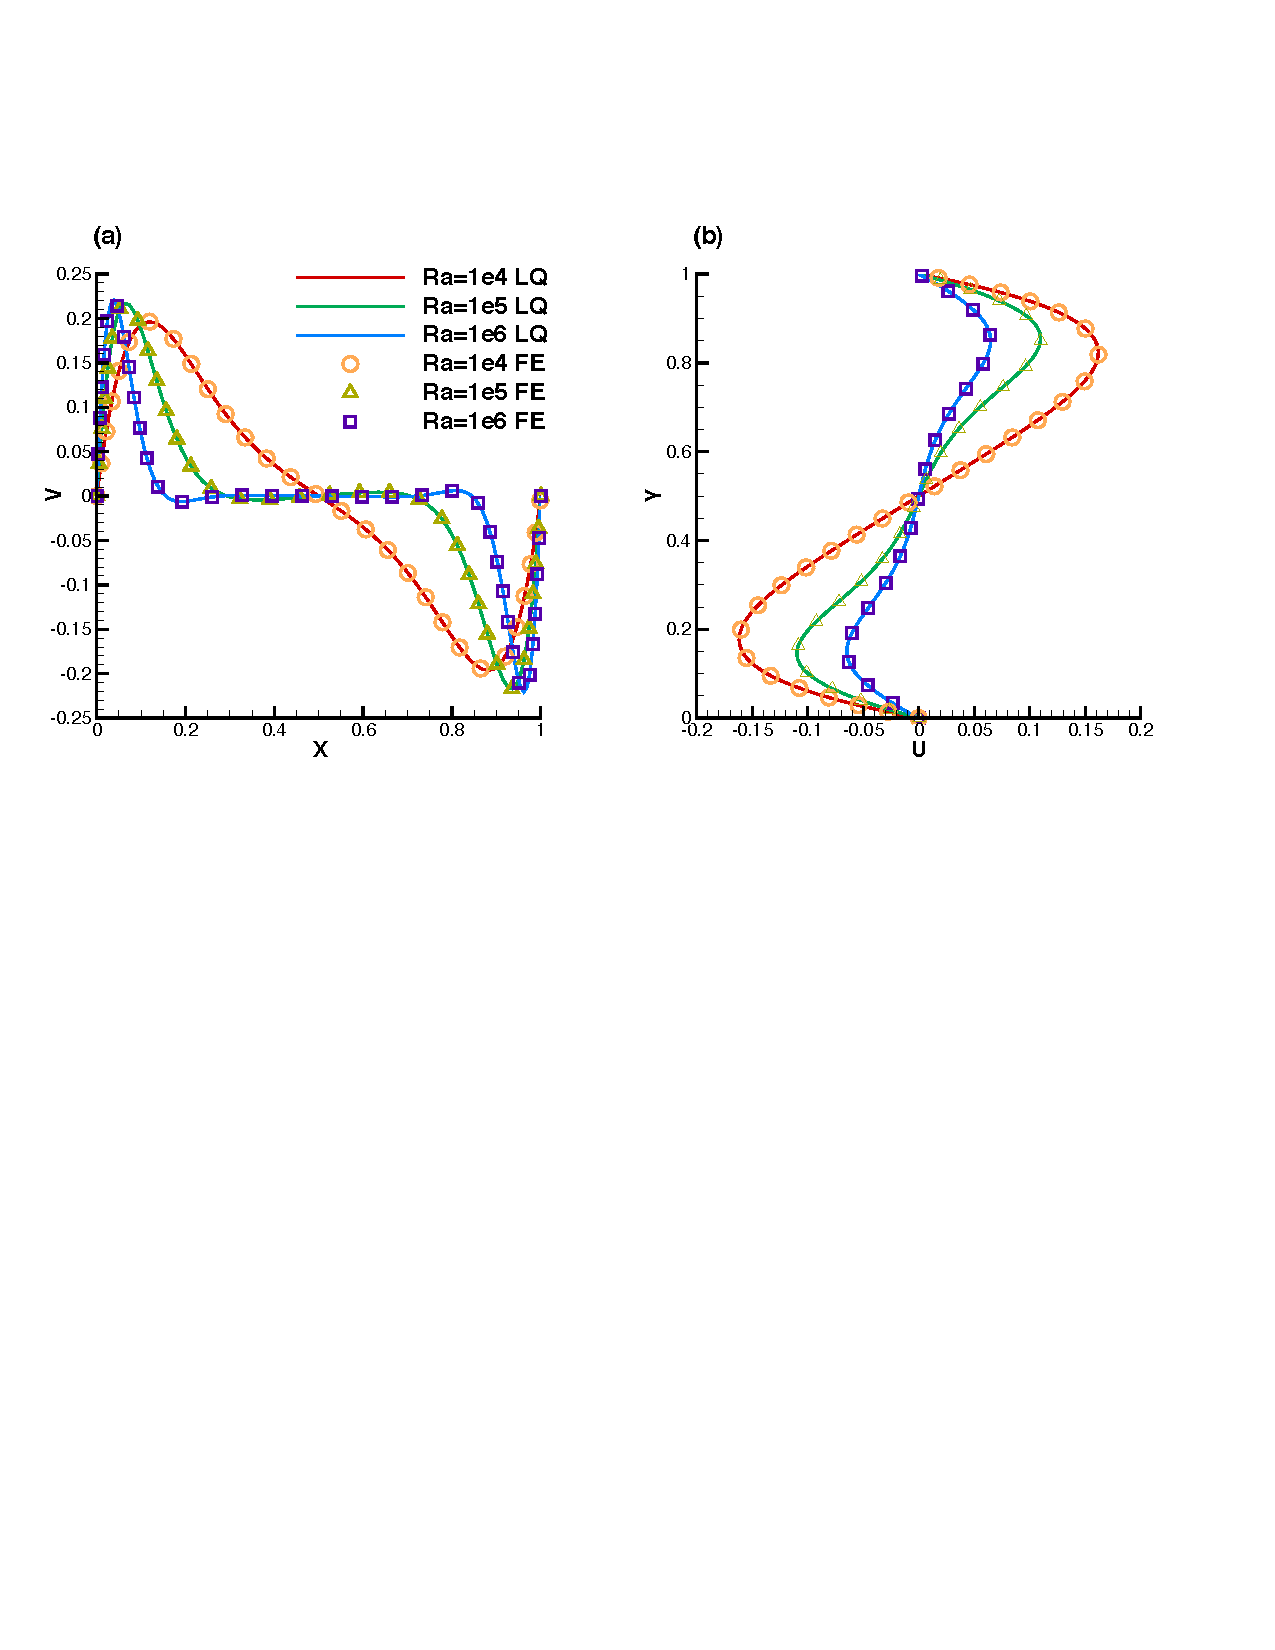
\includegraphics[width=0.98\textwidth]{\figpath/Fig_cap_natconv/Validation_Uprofile_LQ} 
	\end{center}
	\caption{Natural convection of air in a differentially heated cavity for $Ra$ ranging from $10^4$ to $10^6$ and $\Pr = 0.71$. (a) Transversal velocity profile along the  horizontal symmetry lines. (b) Longitudinal velocity profile along the vertical symmetry lines. Numerical results obtained using the present Newton method (symbols) with a mesh resolution of $M=80$; comparison with the spectral-accurate simulations by \cite{LeQuere91} (solid lines).}
	\label{fig-T1-prof}
\end{figure}

The influence of the imposed temperature difference $\delta T$ on the boundary layers are well illustrated in Fig.  (\ref{fig-T1-prof}).
Eq. (\ref{eq-corr-Low-Pr}) indicates a decreasing thickness of the boundary layer for an increasing value of $\Ray$. 
For $\Ray = 10^6$ a viscous boundary layer with a dimensionless thickness of order of $\delta_\nu \sim 0.02$ should be present close to the vertical walls.
Accordingly, the mesh resolution should allow to capture these structures.
A mesh convergence analysis shows a reasonable relative error (lower than $3\%$) from a $80 \times 80$ grid resolution.
Also, from $\Ray = 10^5$ the fluid in the core of the cavity is relatively stagnant and thermally stratified.
This indicates that for $\Ray < 10^5$, the heat transfer is dominated by the bulk heat transfer, while for $\Ray \geq 10^5$ the heat transfer is boundary layer heat transfer.

Tab. (\ref{tab-valid-natconv}) offers a quantitative assessment of the accuracy of the present Newton method. 
The values of $u_{max}$  and its location $Y$ are compared to reference values from \cite{LeQuere91}. 
The Newton method gives results very identical to reference values, with a relative difference less than $0.01 \%$ for the steady and the unsteady codes. 
The characteristics-Galerkin method is less accurate, but still offers reasonable agreement with reference values, within 2$\%$ relative error. 
We also recall that the characteristics method needs a very small time step for refined meshes ($\delta t = 8\cdot 10^{-5}$ for $M=80$), while the Newton method allows larger time steps ($\delta t = 1$ for $M=80$). % and consequently, converges faster to a steady state.
%It is worth noting, that the steady and the unsteady codes provide quasi-identical results.
\begin{table}%[!h]
	\begin{center}
		\begin{tabular}{|l|c|l|l|}
			\hline
			\multicolumn{2}{|l|}{Run} & $u_{max}$ at x=$0.5$ (error) & $Y$ (error) \\
			\hline
			Reference values & spectral & 0.0648344           & 0.850 \\ \hline
			Char-Galerkin       &$M=80$ & 0.0662229 (2.14 $\%$) & 0.856160 ( 0.72 $\%$) \\ \hline
			\cite{dan-2014-JCP}              &$M=80$ & 0.0650082 (0.26 $\%$) & 0.849906 ( 0.01 $\%$) \\ \hline
			Newton (Steady)        &$M=80$ & 0.0648297 (0.007 $\%$) & 0.850394( 0.05 $\%$) \\ \hline
			Newton (Unsteady)        &$M=80$ & 0.0648296 (0.007 $\%$) & 0.850532 ( 0.06 $\%$) \\ \hline
		\end{tabular}
	\end{center}
	\caption {Natural convection of air in a differentially heated cavity for $Ra = 10^6$ and $\Pr = 0.71$. Maximum value $u_{max}$ of the horizontal velocity profile at mid-domain ($x=0.5$) and location $Y$ of this maximum. Comparison to reference values by \cite{LeQuere91}.}
	\label{tab-valid-natconv}
\end{table}

\subsection{Differentially heated cavity with inner heated square} \label{sub-2D-OBSTACLE}

\begin{figure}
	\begin{center}
		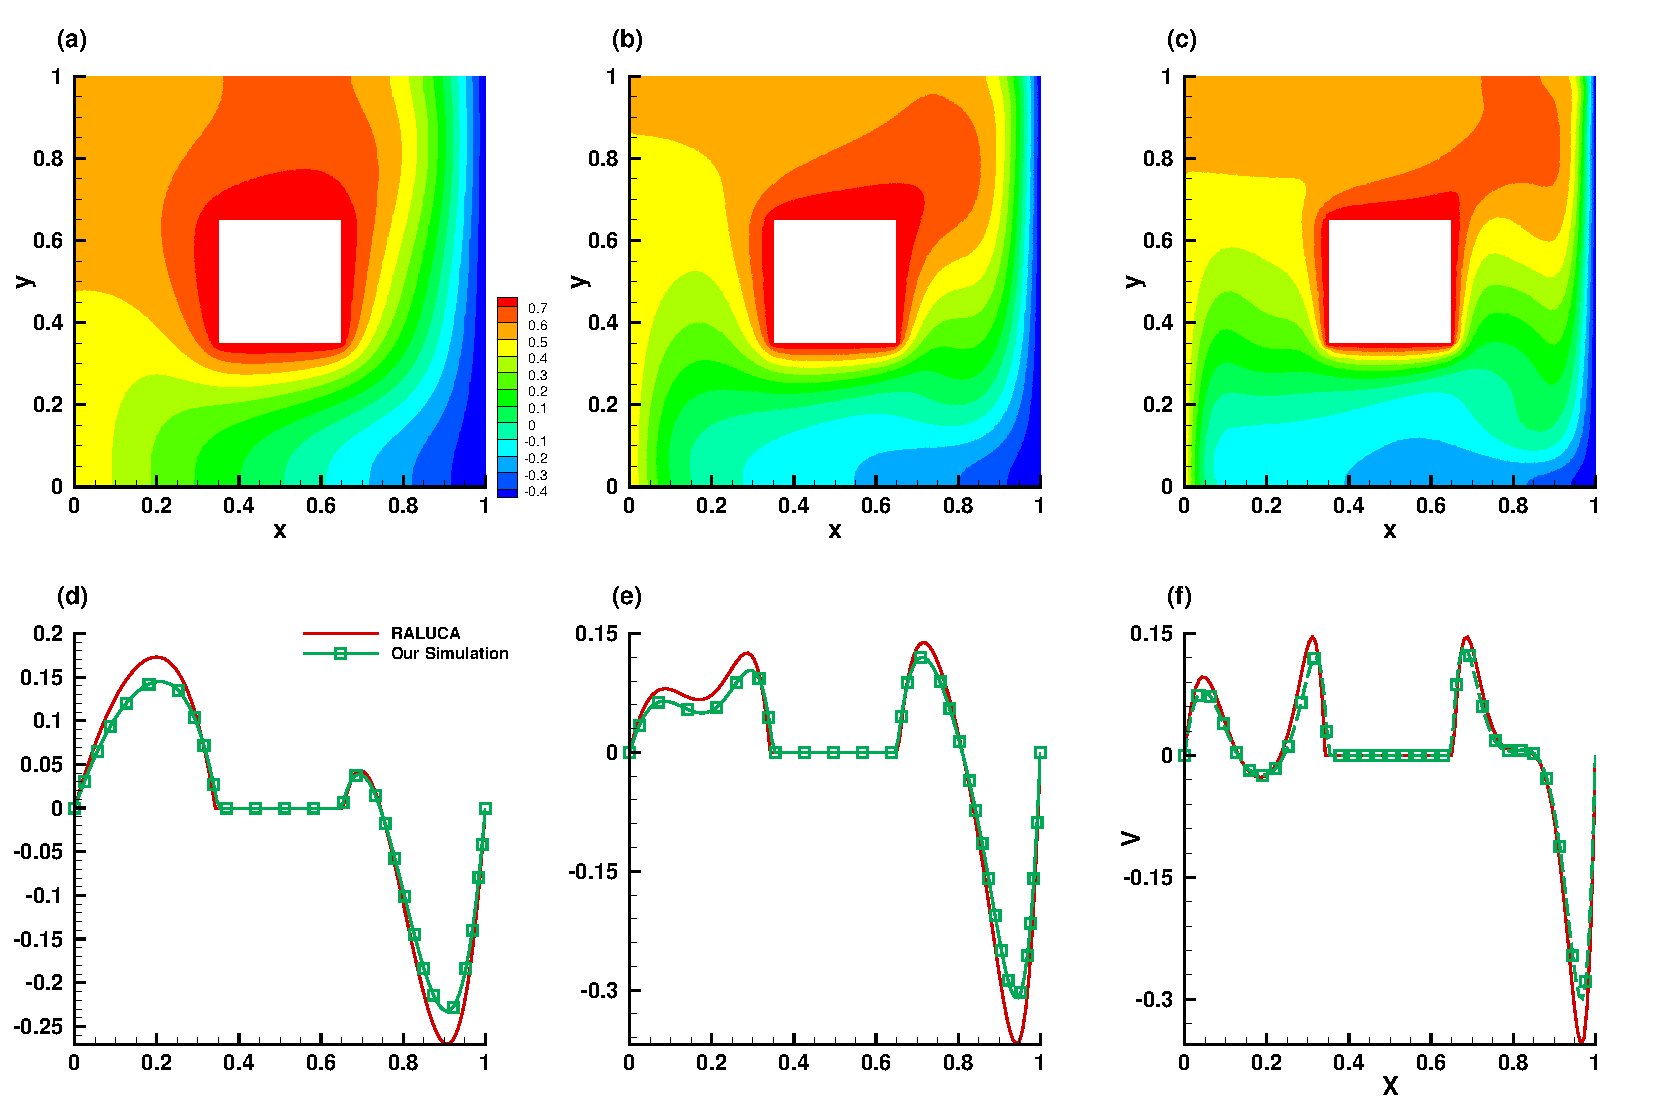
\includegraphics[width=\textwidth]{\figpath/Fig_cap_natconv/STA_validation_obstacle_2} 
	\end{center}
	\caption{Natural convection of air in a differentially heated cavity with inner heated square for $Ra = 10^6$. Temperature field (a) and transversal velocity profile along the  horizontal symmetry lines (b). Results obtained using the present Newton method (red solid line), with mesh resolution $M=80$; comparison with the finite difference code of \cite{Raluca2013}.}
	\label{fig-obst-2D}
\end{figure}

Thermally driven cavity including heated square obstacle is computed in this section.
We consider the same configuration presented in sec. \ref{sub-diff-heated} and a square involving isothermal boundary condition is added between the initial set up.
This kind of basic configuration could be representative of telecommunication outdoor cabinet applications, in which the use of passive cooling solutions have begun to be more and more investigated.
Indeed, inside an outdoor cabinet, electronic equipments generate heat when active and the study of the flow structures within the enclosure have attracted some considerations at the example of the experimental and numerical study of \cite{Raluca2013}.
Simplified model of cavity with rectangular heated obstacles have been investigated by \cite{Raluca2013} and will be reproduced in this section to test the robustness of our numerical algorithm.

A linear distribution of the temperature is imposed initially in the motionless air inside the cavity.
The obstacle is maintained at a dimensionless hot temperature $\theta_h = 0.8$ with a no-slip boundary condition for the velocity.
The solutions for $Ra = 10^4$, $Ra = 10^5$, $Ra = 10^6$ and $Pr = 0.71$ are compared with the result obtained by \cite{Raluca2013} who used an immersed boundary method with a FD code using high order schemes for time and spatial discretization.

The temperature distribution in the cavity when the steady-state is reached, for each of the three $\Ray$ number computed, are shown in panels (a) to (c) of Figs. \ref{fig-obst-2D}.
The temperature gradient gives rise to a clockwise circulation and when $\Ray$ is increased, vertical thermal boundary layers form distinctly along the differentially heated sidewalls and the obstacle.
Consequently, 
higher is the Rayleigh number the more the hot temperature in the center of the domain is advected by the natural convection flow into the cold part of the cavity. 
Worth noting is the fact that at $\Ray = 10^6$ in panels (c) and (d), a stagnant fluid with a stratified temperature forms in a small portion of the fluid between the cold wall and the obstacle.

A more accurate validation is given in panels (d) to (f) of Fig. (\ref{fig-obst-2D}).
The transversal velocity profiles along the x-axis are plotted and compared with the numerical data of \cite{Raluca2013} for each of the three $\Ray$ number investigated. 
A good agreement can be observed with a relatively small differences between the extremum of the velocity while the trends of the velocity profile match well.

We have demonstrated in this part that the proposed Newton method offers an efficient way to solve the Navier-Stokes-Boussinesq system of equations for natural convection of air evolving a linear expression of $f_B(\theta)$.
A further difficulty will be introduced in the next section when a non-linear expression of the body force is defined since natural convection of water is of interest.
%We can conclude from this section that the proposed Newton method offers an efficient way to solve the Navier-Stokes-Boussinesq system of equations for natural convection. After this validation, we test in the following section the capability of the method to deal with phase-change, introducing nonlinearity in the momentum and the energy equations.

\section{Natural convection of water in a two dimensional square cavity}\label{sec: natconv-water}
We investigate in this section the natural convection of water in a differentially heated cavity. 
A further difficulty is taken into account compared to the previous validation by introducing non-linear variation of the density in the buoyancy force.
Pure water involve actually non-linear density variation for $T< \celsm{10.2}$ with a maximum at $T_m= \celsm{4.0293}$. 
We use below the following density-temperature relationship  proposed in \cite{Gebhart1977}:
\begin{equation}
\rho(T)=\rho_m \left(1 - w \left|T - T_m\right|^q\right),
\end{equation}
with $\rho_m=999.972$ [kg/m$^3$], $w=9.2793\cdot 10^{-6}$ [($^\circ C)^{-q}$], and $q=1.894816$.
The bouyancy term $f_B = g(\rho_\vref-\rho)/\rho_\vref$ appearing in eq. (\ref{eq-momentum-conserv})  becomes after scaling:
\begin{equation}
f_B(\theta) = \frac{\Ray}{\Prd \, \Rey^2} \frac{1}{\beta \delta T}\, \frac{\rho(\theta_f)-\rho(\theta)}{\rho(\theta_f)},
\label{eq-fBnonlin}
\end{equation}
where $\beta=(1/\rho_m) \left(d\rho/dT\right)$ is the thermal expansion coefficient with the value \cite{Scanlon2004} $\beta=6.91 \cdot 10^{-5}$ [(K)$^{-1}$].

We simulate a differentially heated cavity of height $H = 0.38 m$ filled with liquid pure distilled water.
This problem was investigated experimentally and numerically in \cite{Giangi-2000,Kowalewski-1999,Kowalewski-2003}.
The height $H$ of the cavity is considered as a length scale of the problem $L_{ref} = H$. 
We choose $T_{ref} = T_h - T_c$ in order to compare our simulation with the numerical results of \cite{Kowalewski-2003},
and define the following scaling:
\begin{equation}
   V_{ref} = \frac{\nu_l}{H} 
   \quad \Longrightarrow \quad t_{ref} = \frac{\nu_l}{H^2}
   \quad \Longrightarrow \quad \Rey = 1.
\end{equation} 
The non-dimensional parameters describing the problem result from the physical properties of water in Tab. \ref{tab-param-phys-air}: $\Ray=2.518084\cdot 10^{6}$ and $\Pr=6.99$. %  (see also \cite{Kowalewski-2003} for physical details). % and $\Ste = 6.99$.

The initial temperature is linearly distributed with a hot temperature $T_h =\celsm{10}$ at the left wall and a cold temperature $T_c=T_f=\celsm{0}$ at the right wall, corresponding to dimensionless thermal boundary condition $\theta_h = 1$ and 
$\theta_c = 0$. The top and the bottom of the cavity are adiabatic and no-slip boundary condition $\vec u = 0$ is used for the velocity.

The Temperature field of the steady state is presented in Figure \ref{fig-T1w-isoT}a and a more accurate comparison of the temperature profile along the horizontal symmetry line is given in Figure \ref{fig-T1w-isoT}b. 
The isoline $\theta = \theta_m$, corresponding to the line of maximum density is presented in Figure \ref{fig-T1w-isoT}a by dashed line.
Indeed, due to the anomalous thermal variation of water density, two recirculating zones are formed in the flow: a lower (abnormal) recirculation  in the vicinity of the cold wall where $\theta<\theta_m$ and an upper (normal) one where the density decreases with temperature ($\theta>\theta_m$).

The temperature profile $\theta(x)$ along the horizontal symmetry line of the cavity is in good agreement with the numerical results   of \cite{Kowalewski-2003} obtained with FV and FD codes (FLUENT and FRECONV3V), commonly used in the heat transfer community. Differences are visible in the vicinity of the maximum density line, region where our mesh is well refined to capture the separation line between the two recirculation zones. It should be noted that the FLUENT simulations in \cite{Kowalewski-2003} are performed with a fixed uniform grid with $380\times380$ nodes, while our adapted grid has only 8751 vertices (17257 triangles).

\begin{figure}
	\begin{center}
		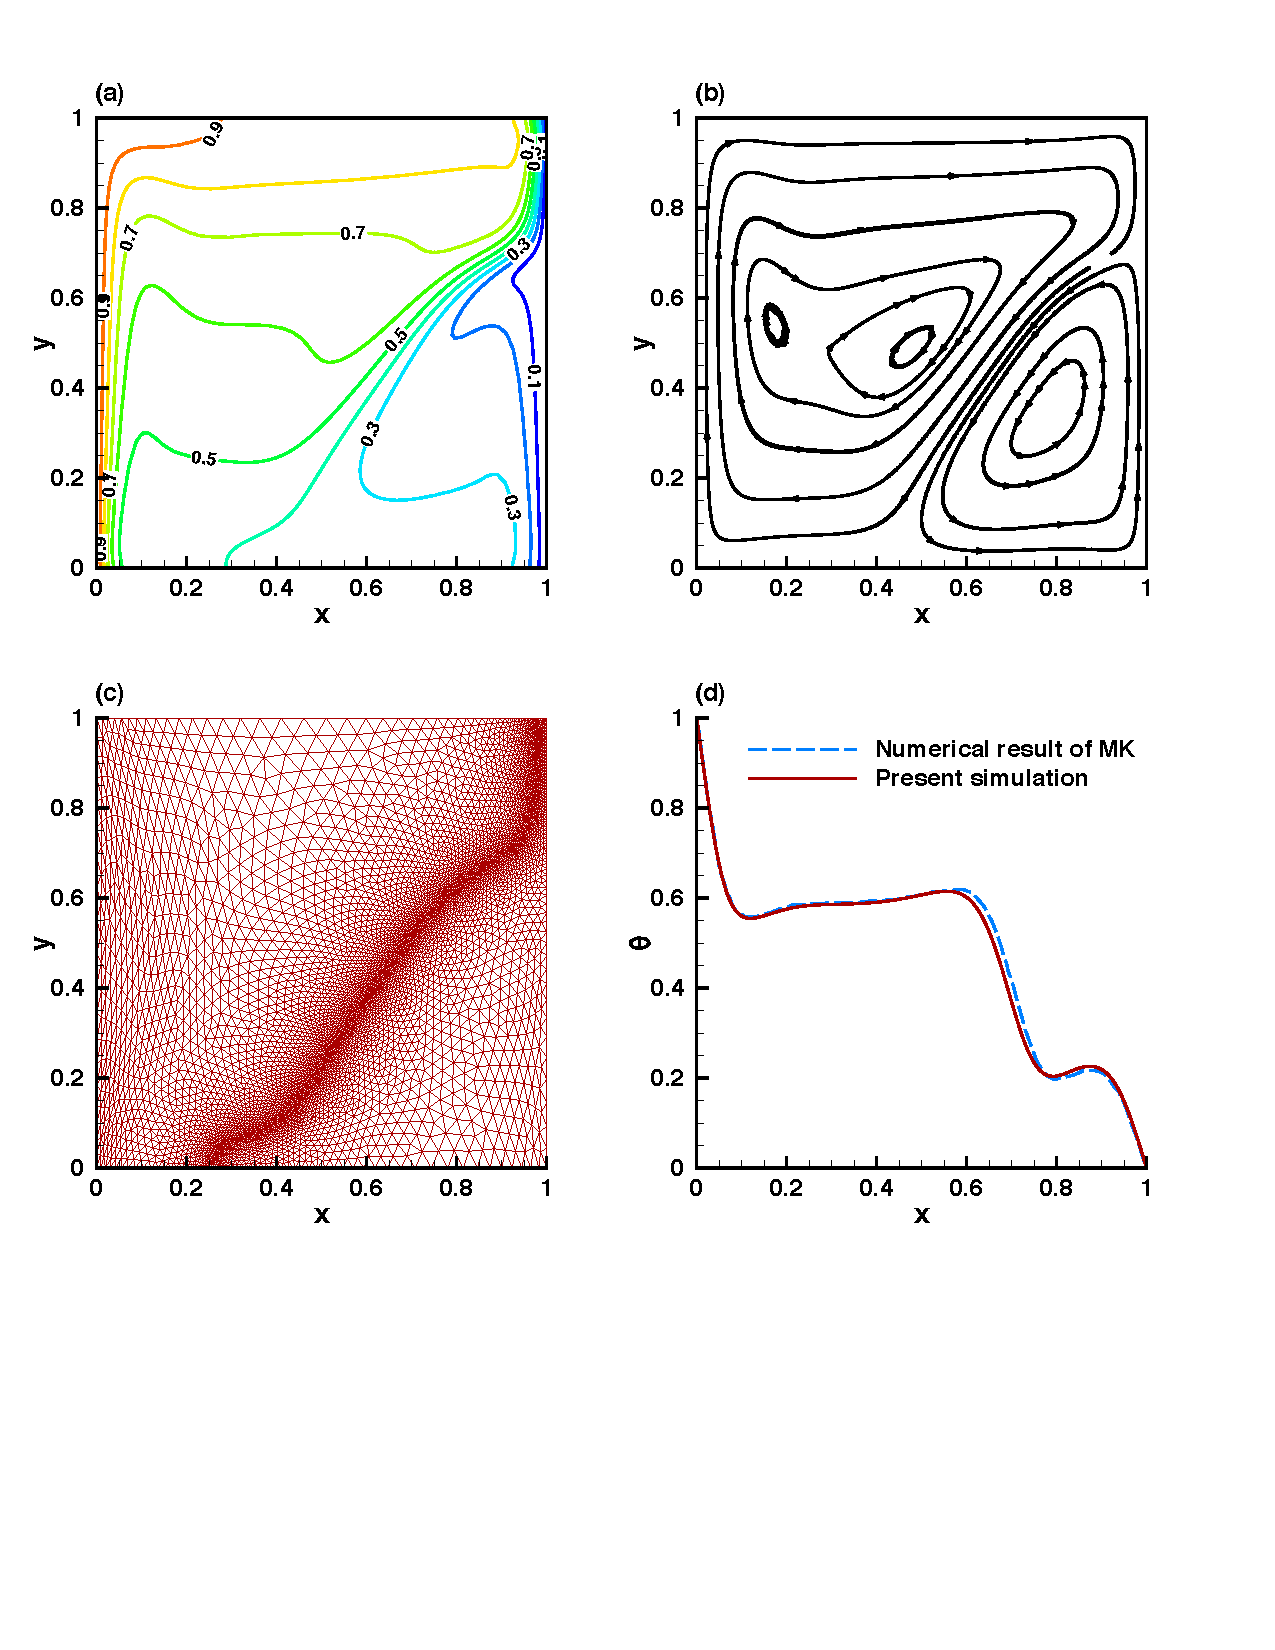
\includegraphics[width=0.98\textwidth]{\figpath/Fig_cap_natconv/WATER_convec_valid}
	\end{center}
	\caption{Natural convection of water in a differentially heated cavity with non-dimensional parameters: $\Ray=2.518084\cdot 10^{6}$ and $\Pr=6.99$. (a) iso-line of the temperature at the steady state. (b) Streamline of the steady flow. (c) Illustration of the mesh adaptivity: The mesh is refined along the dimensionless temperature iso-line $\theta = 0.4$ due to the density variation. (d) Temperature profile along the horizontal symmetry line. Comparison with the numerical results of \cite{Kowalewski-2003}.}
	\label{fig-T1w-isoT} % label should be placed after the caption
\end{figure}

\section{Natural convection of air in a three dimensional cavity using FFDDM}\label{sec: natconv-air-3D}

\subsection{Natural convection in a differentially heated cube cavity}
We present in this section some 3D simulations using ffddm.

%A schematic model of the problem is displayed in figure \ref{fig-3Dmesh} a).
The Prandtl number is $0.71$ and three Rayleigh numbers are considered:  $\Ray=10^4$, $\Ray=10^5$, $\Ray=10^6$. The walls are rigid and impermeable. The vertical walls at $x=0$ and $x=1$ are isothermal and have different temperatures $T_h=0.5$ and $T_c=-0.5$ respectively. The remaining walls are considered adiabatic. % Figure \ref{fig-3Dmesh} b) shows the present three dimensional grid.
%\begin{figure}%[!htbp]
%\begin{minipage}{0.45\linewidth}
%\begin{center}
% {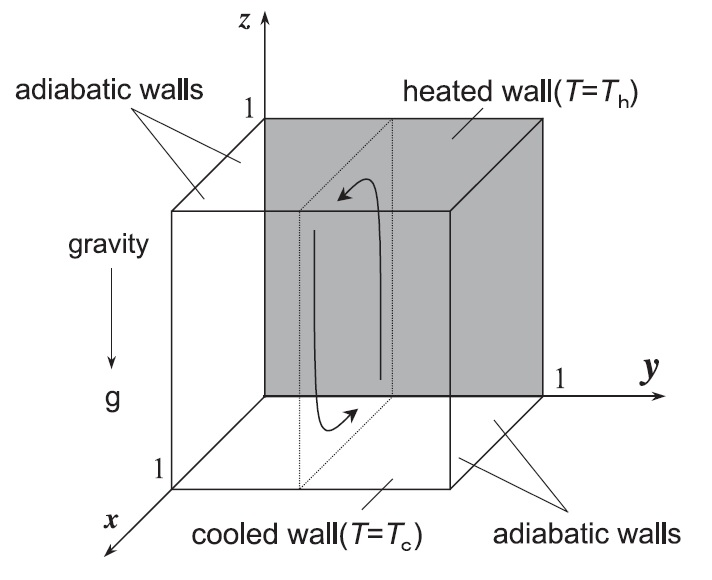
\includegraphics[width=1.\textwidth]{\figpath/Fig_cap_natconv/3D_scema.jpg}}\\
% a)
%\end{center}
%\end{minipage}\hfill
%\begin{minipage}{0.45\linewidth}
%\begin{center}
% {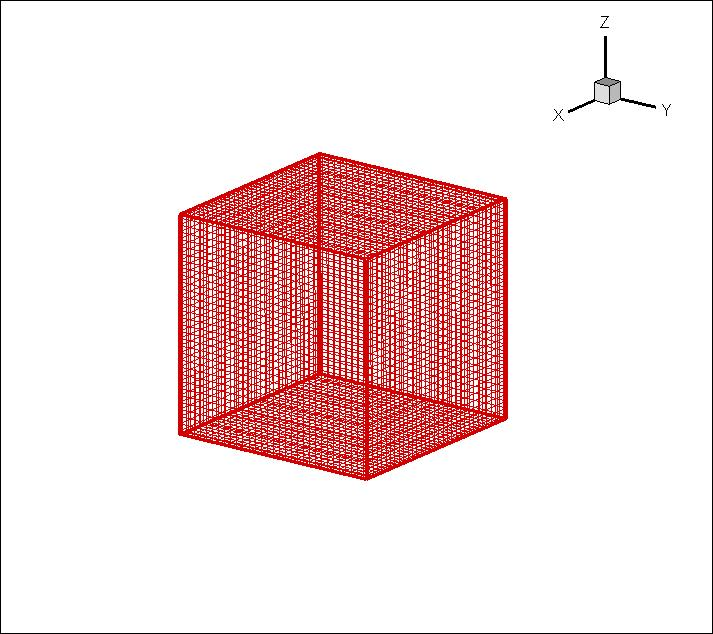
\includegraphics[width=1.\textwidth]{\figpath/Fig_cap_natconv/mesh3D.jpg}}\\
% b)
%\end{center}
%\end{minipage}
%\caption{(a) Schematic model for the natural convection in a cubic cavity; (b) present 3D uniform mesh.}
%\label{fig-3Dmesh}
%\end{figure}
 
Our result were obtained for uniform grids of $  40 \times 40 \times 40$ and is compared with \cite{Wakashima-2004} who used a forth order finite difference method, with a vorticity-stream function formulation with different uniform meshes of  $120 \times 120 \times 120 \times 10$ grid nodes. 
This result obtained with sequential algorithm is also used to validate the 3D simulations using ffddm.

Fig. \ref{fig-3DT} shows the temperature field for each of the three Rayleigh numbers $\Ray = 10^4$, $\Ray = 10^5$, $\Ray = 10^6$, at the mid section (y=0.5).
On the left we display the numerical results of \cite{Wakashima-2004} and on the right ou results.
The comparison with the benchmark solution exhibits a fairly good agreement.

The parallel algorithm used with ffddm is compared with the sequential algorithm.
$\mathcal{L}_2$-norm and $\mathcal{L}_\infty$-norm of the velocity and the temperature are computed and reported in Tab. \ref{tab-T1} for Rayleigh number varying from $10^4$ to $10^6$.
The difference between both algorithm is of order of $10^{-6}$.
Moreover, we do not observe a large variation of the error when the number of subdomains is increased.
The number of subdomain vary from $28$ to $70$ for $1.8$ millions of unknown.

\begin{table}[!h]
	\begin{center}
		\begin{tabular}{|*{6}{c|}}
			\hline
			 Ra & nb proc                     & $||u||_{2}$                        & $||u||_{\infty}$                & $||T||_{2}$              & $||T||_{\infty}$\\ \hline \hline
			\multirow{4}{*}{$10^4$} & 28 & $1.12496 \cdot 10^{-6}$ & $3.1 \cdot 10^{-6}$ & $ 3.09966 \cdot 10^{-6} $ & $7 \cdot 10^{-6}$ \\% \hline
			\cline{2-6}
			& 42 & $1.53698 \cdot 10^{-6}$ & $5.1 \cdot 10^{-6}$ & $ 3.23352 \cdot 10^{-6} $ & $8 \cdot 10^{-6}$ \\ \cline{2-6} %\hline 
			& 56 & $1.55576 \cdot 10^{-6}$ & $5.1 \cdot 10^{-6}$ & $ 3.4342 \cdot 10^{-6} $ & $8 \cdot 10^{-6}$  \\ \cline{2-6} %\hline
			& 70 & $1.25622 \cdot 10^{-6}$ & $3.6 \cdot 10^{-6}$ & $ 3.56048 \cdot 10^{-6} $ & $8 \cdot 10^{-6}$ \\ \hline \hline
			\multirow{4}{*}{$10^5$} & 28 & $1.73254 \cdot 10^{-6}$ & $6.1 \cdot 10^{-6}$ & $ 2.40467 \cdot 10^{-6} $ & $7 \cdot 10^{-6}$ \\% \hline
			\cline{2-6}
			& 42 & $2.84973 \cdot 10^{-6}$ & $7.78 \cdot 10^{-6}$ & $ 3.53003 \cdot 10^{-6} $ & $9 \cdot 10^{-6}$ \\ \cline{2-6} %\hline 
			& 56 & $3.00832 \cdot 10^{-6}$ & $7.39 \cdot 10^{-6}$ & $ 4.17769 \cdot 10^{-6} $ & $1.1 \cdot 10^{-5}$  \\ \cline{2-6} %\hline
			& 70 & $3.68118 \cdot 10^{-6}$ & $9 \cdot 10^{-6}$ & $ 4.70846 \cdot 10^{-6} $ & $1.2 \cdot 10^{-5}$ \\ \hline \hline
			\multirow{4}{*}{$10^6$} & 28 & $6.61804 \cdot 10^{-6}$ & $1.826 \cdot 10^{-5}$ & $ 3.46504\cdot 10^{-6} $ & $1.1 \cdot 10^{-5}$ \\% \hline
			\cline{2-6}
			& 42 & $5.93966 \cdot 10^{-6}$ & $1.5 \cdot 10^{-5}$ & $ 3.98082 \cdot 10^{-6} $ & $1.2 \cdot 10^{-5}$ \\ \cline{2-6} %\hline 
			& 56 & $7.05144 \cdot 10^{-6}$ & $1.9247 \cdot 10^{-5}$ & $ 5.0044 \cdot 10^{-6} $ & $2 \cdot 10^{-5}$  \\ \cline{2-6} %\hline
			& 70 & $6.02152 \cdot 10^{-6}$ & $1.68 \cdot 10^{-5}$ & $ 4.50094 \cdot 10^{-6} $ & $1.8 \cdot 10^{-5}$ \\ \hline
		\end{tabular}
	\end{center}
	\caption {3D differentially heated cavity. Comparison between sequential and ffddm algorithm for uniform grids of $40 \times 40 \times 40$ }
	\label{tab-T1}
\end{table}


\begin{figure}%[!htbp]
\begin{minipage}{\linewidth}
\begin{center}
 {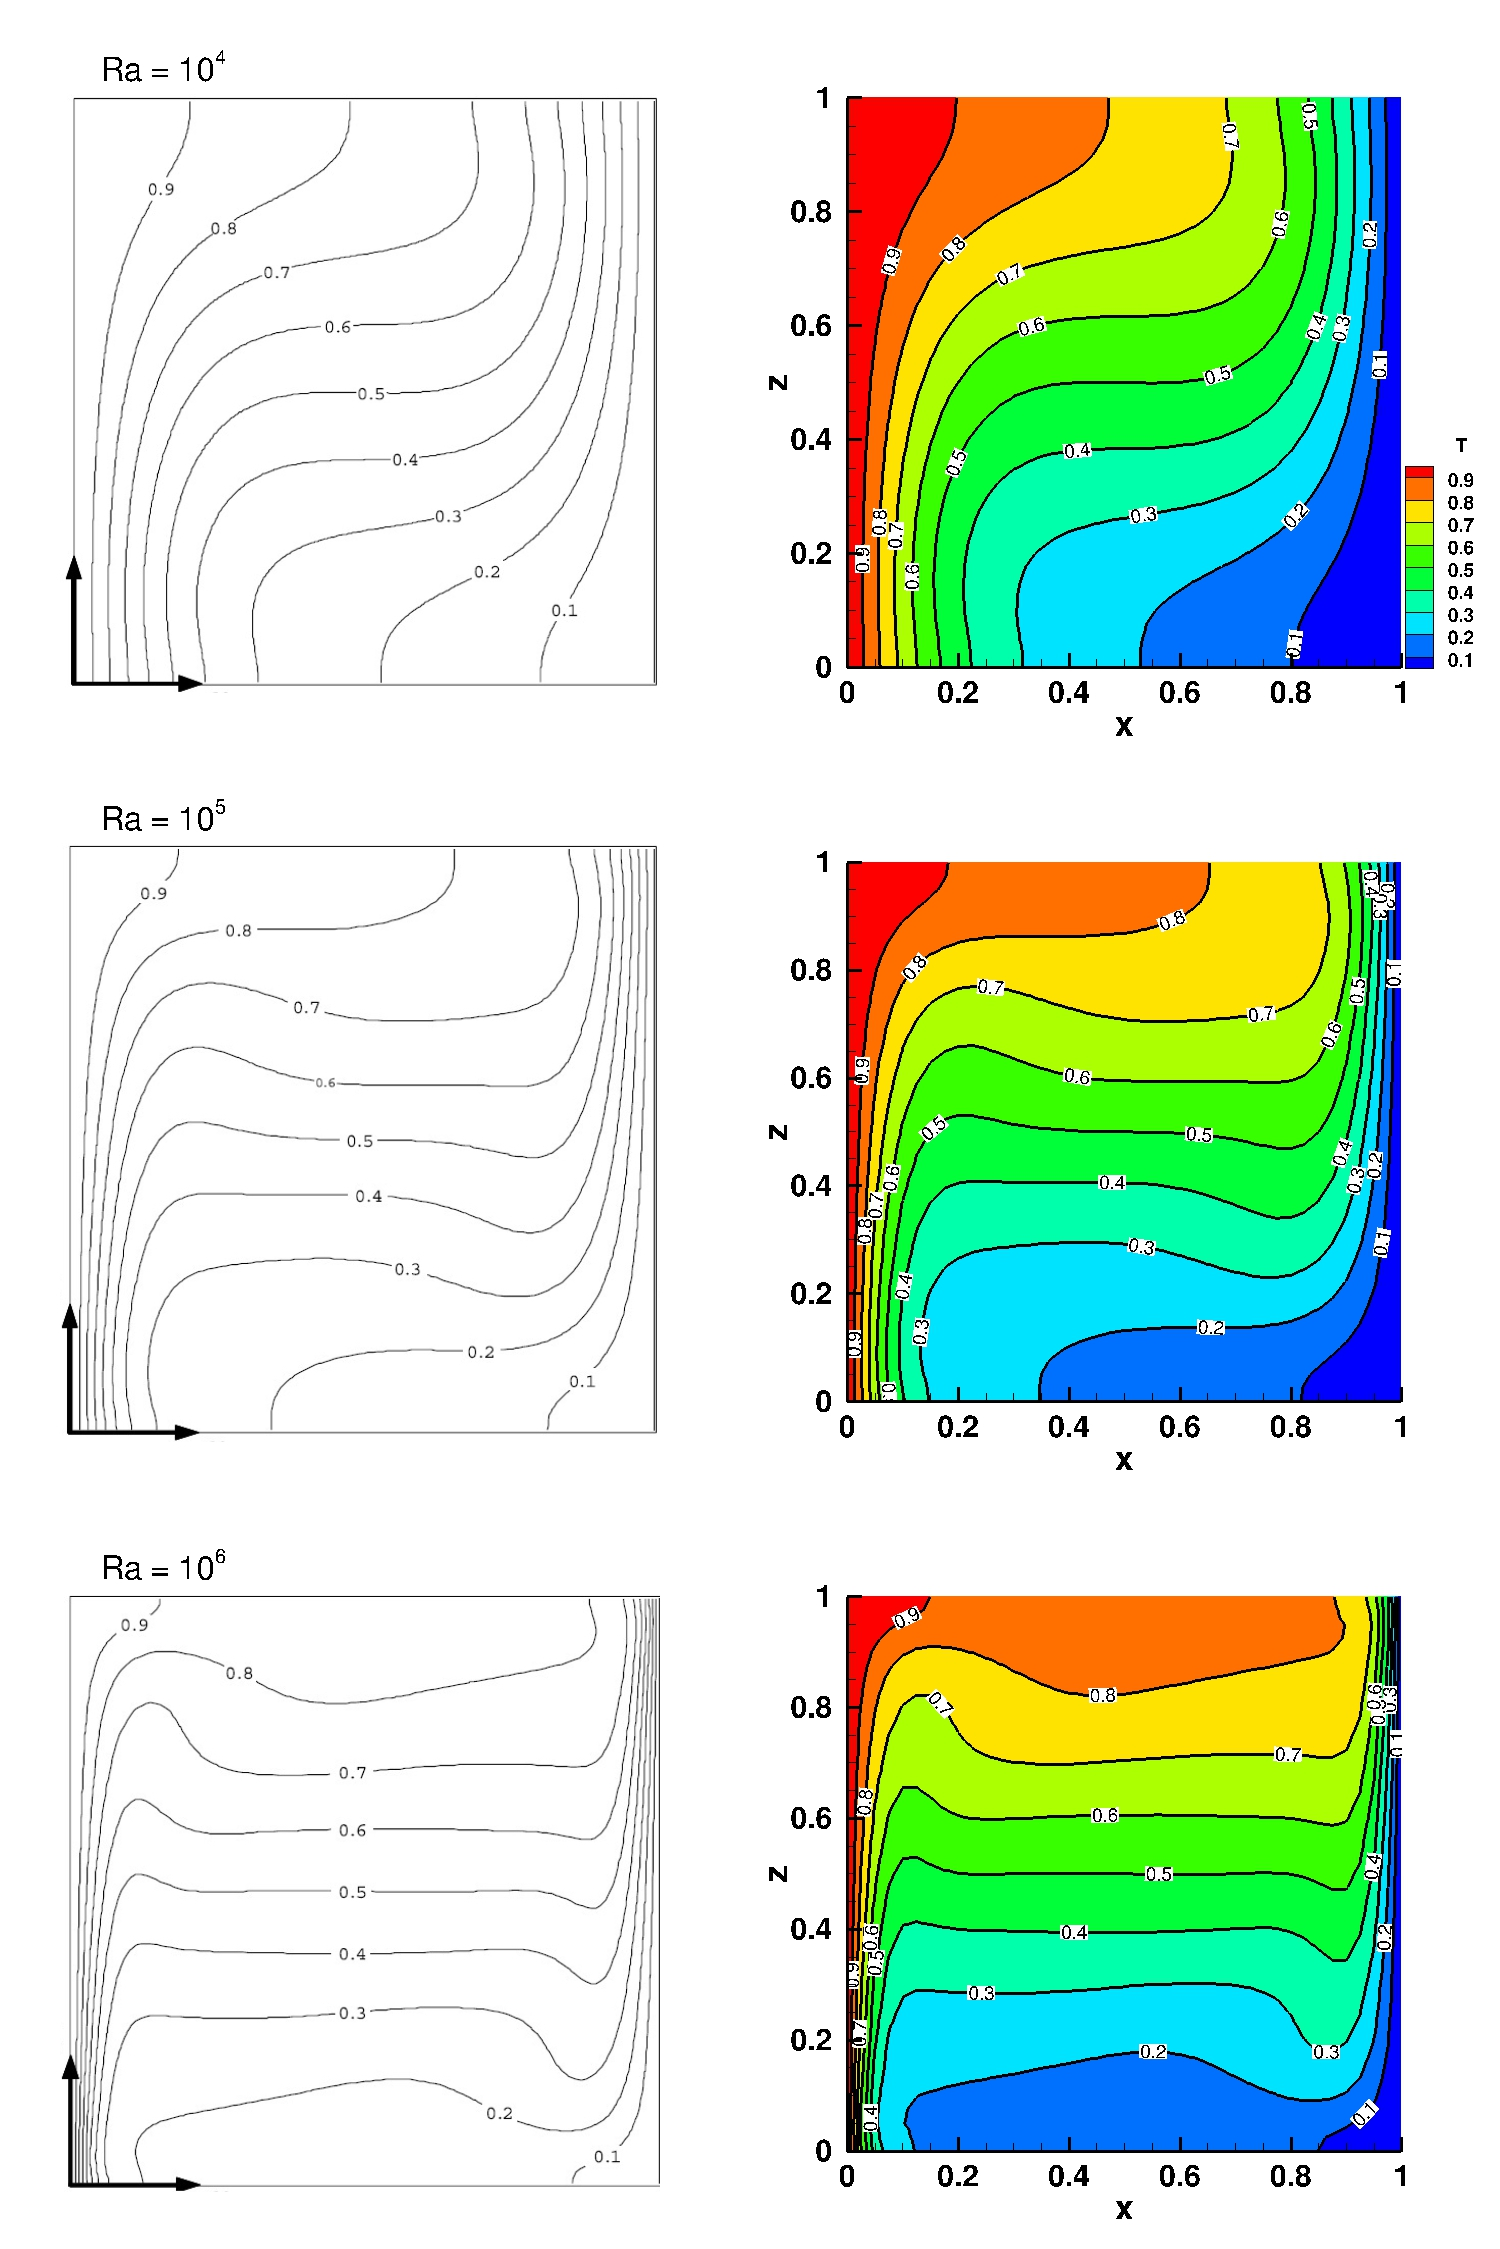
\includegraphics[width=\textwidth]{\figpath/Fig_cap_natconv/Validation_3D_seq_T1}}
\end{center}
\end{minipage}
\caption{3D differentially heated cavity. Temperature contours at the mid-plane of ($y=0.5$); comparison with the results of \cite{Wakashima-2004} (left images). }
\label{fig-3DT} 
\end{figure}


%  1 proc    MatLoc  MatCS   PREC    GMRES   CSolve
%  2 48      6186.33 108.385 61.0397 473.66  2.97339
%  3 96      2468.68 116.805 33.2671 283.099 3.03667
%  4 128     1814.26 116.464 45.5823 237.853 2.74235
%  5 192     1111.5  116.601 25.7295 169.174 2.96447
%  6 240     889.422 123.724 20.8664 146.539 3.03816
%  7 320     674.204 123.723 16.5842 114.346 3.0098
%  8 400     614.418 136.961 14.4055 107.422 3.14586

\subsection{Natural convection in a cube with an inner heated obstacle}\label{sub-OBSTACLE-3D}

The three-dimensional natural convection induced by a temperature difference between a cold outer cubic enclosure is investigated in this section.
Sequential and parallel computation using ffddm are carried out and compared together.

Different Rayleigh numbers varying in the range of $10^4 -10^6$ are considered. The temperature field for $Ra = 10^4$ is reported in Figure \ref{fig-obstacle-Ra1e4} and the Table \ref{tab-T2} shows the error between the sequential and the parallel computation.

\begin{figure}%[!htbp]
\begin{center}
\begin{minipage}{\linewidth}
 {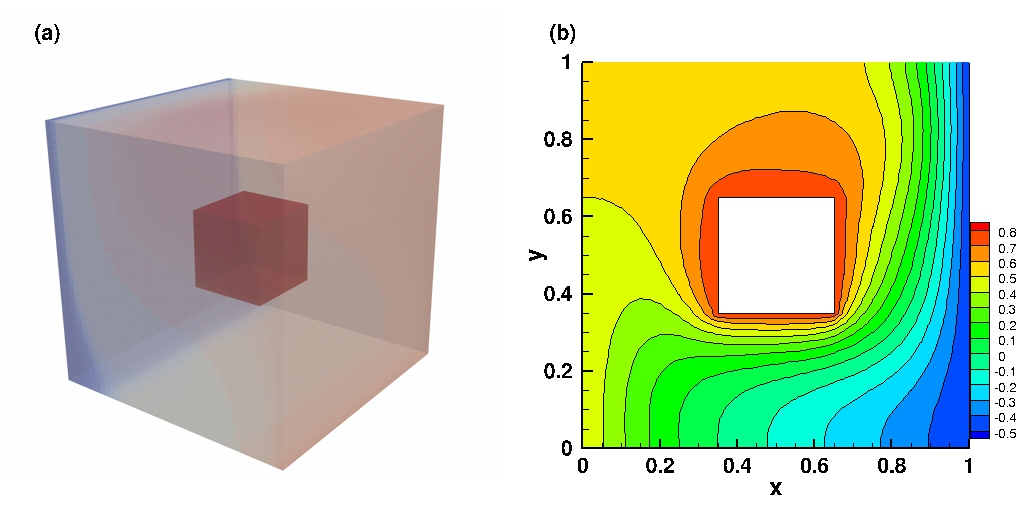
\includegraphics[width=0.98\textwidth]{\figpath/Fig_cap_natconv/3D_OBSTACLE_field}}
\end{minipage}
\end{center}
\caption{3D convection in a cube with an inner heated cube. Temperature fields for $Ra = 10^4$.}
\label{fig-obstacle-Ra1e4} 
\end{figure}

\begin{table}[!h]
	\begin{center}
		\begin{tabular}{|*{7}{c|}}
			\hline
			 Ra & nbseg & nb proc                     & $||u||_{2}$                        & $||u||_{\infty}$                & $||T||_{2}$              & $||T||_{\infty}$\\ \hline \hline
			\multirow{12}{*}{$10^4$} & \multirow{4}{*}{40} & 28 & $0.00087137$ & $0.0058298$ & $ 0.0022491 $ & $0.01592$ \\
			\cline{3-7}
			& & 42 & $0.000870796$ & $0.0058292$ & $ 0.00224866 $ & $0.015921$ \\ \cline{3-7} %\hline 
			& & 56 & $0.000870646$ & $0.0058293$ & $ 0.00224788 $ & $0.015921$  \\ \cline{3-7} %\hline
			& & 70 & $0.000870747$ & $0.0058286$ & $ 0.00224795 $ & $0.015921$ \\ \cline{2-7}
			 & \multirow{4}{*}{60} & 112 & $0.000785593$ & $0.0021$ & $ 0.000858912 $ & $0.010024$ \\% \hline
			\cline{3-7}
			& & 140 & $0.000783164$ & $0.002097$ & $ 0.000865668 $ & $0.010024$ \\ \cline{3-7} %\hline 
			& & 168 & $0.000779419$ & $0.002091$ & $ 0.000858384 $ & $0.010027$  \\ \cline{3-7} %\hline
			& & 196 & $0.000767662$ & $0.00209$ & $ 0.000864693 $ & $0.010019$ \\ \cline{2-7}
			 & \multirow{4}{*}{80} & 224 & $0.000637268$ & $0.001795$ & $ 0.000551538 $ & $0.001661$ \\% \hline
			\cline{3-7}
			& & 238 & $0.000152936$ & $0.000548$ & $ 0.000205031 $ & $0.000634$ \\ \cline{3-7} %\hline 
			& & 252 & $0.000239786$ & $0.000841$ & $ 0.000231648 $ & $0.000661$  \\ \cline{3-7} %\hline
			& & 266 & $0$ & $0$ & $ 0 $ & $0$ \\ \hline 
			\multirow{12}{*}{$10^5$}& \multirow{4}{*}{40} & 28 & $0.0011359$ & $0.0089746$ & $ 0.00401922 $ & $0.020067$ \\% \hline
			\cline{3-7}
			& & 42 & $0.00113742$ & $0.0089788$ & $ 0.00402103 $ & $0.020067$  \\ \cline{3-7} %\hline 
			& & 56 & $0.00113625$ & $0.0089768$ & $ 0.00402081 $ & $0.020063$   \\ \cline{3-7}%\hline
			& & 70 & $0.0011348$ & $0.0089726$ & $ 0.00401999 $ & $0.020065$  \\ \cline{2-7} %\hline
			 & \multirow{4}{*}{60} & 112 & $0.000765582$ & $0.0022345$ & $ 0.00166687 $ & $0.015296$ \\% \hline
			\cline{3-7}
			& & 140 & $0.000763449$ & $0.0022313$ & $ 0.00166143 $ & $0.015257$ \\ \cline{3-7} %\hline 
			& & 168 & $0.000763074$ & $0.0022176$ & $ 0.00166605 $ & $0.015284$  \\ \cline{3-7} %\hline
			& & 196 & $0.000760368$ & $0.0022093$ & $ 0.00167368 $ & $0.015299$ \\ \cline{2-7} 
			 & \multirow{4}{*}{80} & 224 & $0.00051462$ & $0.0016627$ & $ 0.000574467 $ & $0.001794$ \\% \hline
			\cline{3-7}
			& & 238 & $5.17443 \times 10^{-05}$ & $0.0001934$ & $ 0.00018074 $ & $0.0005666$ \\ \cline{3-7} %\hline 
			& & 252 & $8.68245 \times 10^{-05}$ & $0.000319$ & $ 8.11788 \times 10^{-05} $ & $0.000335$  \\ \cline{3-7} %\hline
			& & 266 & $0$ & $0$ & $ 0 $ & $0$ \\ \hline 

		\end{tabular}
	\end{center}
	\caption {3D convection in a cube with an inner heated cube. Comparison between sequential and ffddm algorithm for uniform grids of $40 \times 40 \times 40$ for $Ra = 10^4$ and $80 \times 80 \times 80$ for $Ra = 10^5$}
	\label{tab-T2}
\end{table}

%The study investigated the effect of the inner sphere location on the heat transfer and fluid flow. A schematic of the three-dimensional domain is presented in figure \ref{fig-cerc_3D}. 
%\begin{figure}[!htbp]
%\begin{minipage}{1.\linewidth}
%\begin{center}
% {\includegraphics[width=0.6\textwidth]{\figpath/figs_Raluca_thesis/cap_5/grafic_C3D.jpg}}\\
%\end{center}
%\end{minipage}
%\caption{Computational domain and boundary conditions for a 3D convection problem with a spherical obstacle.}
%\label{fig-cerc_3D} 
%\end{figure}
%
%%The flow and termal fields eventually reach the steady state for all Rayleigh numbers regardless of the sphere location.
%No-slip boundary conditions are imposed on the walls for the velocity field. The walls are isothermal, of temperature $T=0$, while the inner sphere temperature is $T=1$. The flow and thermal fields converge towards a steady state for all Rayleigh numbers.  
%
%Figure \ref{fig-cerc_iso} presents the isotherms and streamlines obtained by \cite{Yoon-2010} for Rayleigh numbers varying from $10^4$ to $10^6$. 
%\begin{figure}[!htbp]
%\begin{minipage}{1.\linewidth}
%\begin{center}
%$Ra=10^4$\\
% {\includegraphics[width=0.5\textwidth]{\figpath/figs_Raluca_thesis/cap_5/grafic_C3D_Ra1e4.jpg}}
%\end{center}
%\end{minipage}
%\begin{minipage}{1.\linewidth}
%\begin{center}
% $Ra=10^5$\\
% {\includegraphics[width=0.5\textwidth]{\figpath/figs_Raluca_thesis/cap_5/grafic_C3D_Ra1e5.jpg}}
%\end{center}
%\end{minipage}
%\begin{minipage}{1.\linewidth}
%\begin{center}
%$Ra=10^6$\\
% {\includegraphics[width=0.5\textwidth]{\figpath/figs_Raluca_thesis/cap_5/grafic_C3D_Ra1e6.jpg}}
%\end{center}
%\end{minipage}
%\caption{3D convection problem with a spherical obstacle. Isotherms and streamlines for three different $Ra$ numbers.  Results of \cite{Yoon-2010}.}
%\label{fig-cerc_iso} 
%\end{figure}
%
%
%%%\clearpage
%
%Figure \ref{fig-cerc_ra6} shows the same maps obtained with our numerical code.  For $\Ray=10^4$, the effect of convection on heat transfer is low forming a weak upward thermal plume on the top of the sphere.  The thermal boundary layer on the bottom part of sphere is thinner than that on the upper side. The circulation in the upper part of the enclosure is more active, resulting in the formation of one inner recirculation cell.
%
%
%For $Ra=10^5$ convection is predominant with respect to conduction,  as shown in figure \ref{fig-cerc_ra6}. A plume forms on top of the inner sphere which gives rise to stronger thermal gradient on the top of the enclosure. The dominant flow is in the upper half of the enclosure, and correspondingly the center of the recirculating cell is located in the upper half. %The flow at the bottom of the enclosure is weak compared with that the middle and top regions suggesting a stratification effect in the lower part of the cavity.
%
%
%For $\Ray=10^6$, the isotherms are distorted  due to the stronger convection effects thus having a stable stratification of isotherms.
%The convection velocity increases with increasing Rayleigh number, the boundary layer behaviour can be seen in the lower part regions of the sphere and the upper part of the enclosure. The plume arising form the sphere separates as it reaches the top wall. The centres of the inner recirculation cells move toward the upper corners. 
%
%
%\begin{figure}[!htbp]
%$Ra=10^4$\\
%\begin{minipage}{0.32\linewidth}
%\begin{center}
% {\includegraphics[width=1.\textwidth]{\figpath/figs_Raluca_thesis/cap_5/Ra1e4_3.jpg}}\\
% \end{center}
%\end{minipage}
%\begin{minipage}{0.32\linewidth}
%\begin{center}
% {\includegraphics[width=1.\textwidth]{\figpath/figs_Raluca_thesis/cap_5/Ra1e4_7.jpg}}\\
%\end{center}
%\end{minipage}
%\begin{minipage}{0.32\linewidth}
%\begin{center}
% {\includegraphics[width=1.\textwidth]{\figpath/figs_Raluca_thesis/cap_5/Ra1e4_9.jpg}}\\
%\end{center}
%\end{minipage}
%
%$Ra=10^5$\\
%\begin{minipage}{0.32\linewidth}
%\begin{center}
% {\includegraphics[width=1.\textwidth]{\figpath/figs_Raluca_thesis/cap_5/Ra1e5_4.jpg}}\\
%\end{center}
%\end{minipage}
%\begin{minipage}{0.32\linewidth}
%\begin{center}
% {\includegraphics[width=1.\textwidth]{\figpath/figs_Raluca_thesis/cap_5/Ra1e5_7.jpg}}\\
%\end{center}
%\end{minipage}
%\begin{minipage}{0.32\linewidth}
%\begin{center}
% {\includegraphics[width=1.\textwidth]{\figpath/figs_Raluca_thesis/cap_5/Ra1e5_9.jpg}}\\
%\end{center}
%\end{minipage}
%
%
%$Ra=10^6$\\
%\begin{minipage}{0.32\linewidth}
%\begin{center}
% {\includegraphics[width=1.\textwidth]{\figpath/figs_Raluca_thesis/cap_5/Ra1e6_3.jpg}}\\
%\end{center}
%\end{minipage}
%\begin{minipage}{0.32\linewidth}
%\begin{center}
% {\includegraphics[width=1.\textwidth]{\figpath/figs_Raluca_thesis/cap_5/Ra1e6_7.jpg}}\\
%\end{center}
%\end{minipage}
%\begin{minipage}{0.32\linewidth}
%\begin{center}
% {\includegraphics[width=1.\textwidth]{\figpath/figs_Raluca_thesis/cap_5/Ra1e6_9.jpg}}\\
%\end{center}
%\end{minipage}
%\caption{3D convection problem with a spherical obstacle. Present study. Isotherms and streamlines for different Rayleigh numbers.}
%\label{fig-cerc_ra6} 
%\end{figure}
%
%We can conclude that the results obtained with our FD+IBM method for the 3D case  are in good agreement with the test case considered, rendering possible the simulation of 3D configurations with obstacles of general geometries.


%\subsection{Note on parameters for ffddm and Newton method}\label{ffddm-param}
%In this section, we only focus on natural or mixed convection, without phase changing. The system of non-linear equations (\ref{eq-weak-all}) is solved using a Newton method. We have tested two ways of solving this non linear problem. Rewriting the problem as 
%$$
%F(U) = 0,
%$$
%Newton method can be implemented in any of the two following ways:\begin{itemize}
%\item Start with initial guess $U^{(0)}$ and compute $W$ from:
%$$
%W = DF(U^{(k)})^{-1}\ F(u^{(k)}).
%$$
%Then, update $U^{(k+1)} = U^{(k)}-W$.
%\item Start with initial guess $U^{(0)}$ and directly compute $U^{(k+1)}$ from:
%\begin{equation}\label{eq:newton_approach}
%U^{(k+1)} = DF(U^{(k)})^{-1}\left( DF(U^{(k)}) U^{(k)} - F(U^{(k)})\right).
%\end{equation}
%\end{itemize}
%We choose the latter \eqref{eq:newton_approach} for several reasons: for example, the right hand side and time-dependent boundary conditions (when applicable) are easier to implement. Moreover, ffddm uses algebraic norms to compute residuals, thus making the norms mesh dependent. It is then natural to use the iterative solver of ffddm with relative tolerance. This relative error is based on the right hand side. In the first case, this norm will decrease so that it is difficult to set up a good criterion. In the latter, we expect very few variations in the amplitude of the successive RHS.
%
%Eventually, at each Newton iteration, we have to solve linear problems of the kind: start with $(u^{(0)},p^{(0)},\theta^{(0)})=(u_n,p_n,\theta_n)$, and find $(u^{(k+1)},p^{(k+1)},\theta^{(k+1)})$ from
%\begin{align*}
%cdt\ u^{(k+1)} + u^{(k)}\nabla u^{(k+1)} + u^{(k+1)}\nabla u^{(k)} &- IRe\Delta u^{(k+1)} + \nabla p^{(k+1)} - IRe\;cc\;\theta^{(k+1)} e_y \\
%&= u^{(k)}\nabla u^{(k)}  + cdt\ u_n, \\
%\nabla\cdot u^{(k+1)} + \epsilon p^{(k+1)} &= 0, \\
%cdt\ \theta^{(k+1)} + u^{(k)}\nabla\theta^{(k+1)} + u^{(k+1)}\nabla\theta^{(k)} -IPr\Delta \theta^{(k+1)} &= u^{(k)}\nabla\theta{(k)} + cdt\ \theta_n
%\end{align*}
%
%$\epsilon$ is a penalty term with very small value ($\epsilon=1.e-7$), $cdt$ is $1/{\delta t}$ (resp. 0) in the unsteady problem (resp. stationary cases). $cc=1$ for unsteady problems. For stationary problems, we solve the problems for different values of $cc$, from $0$ to $1$. The reason is that the original problem ($cc=1$) can be difficult to approximate with Newton's method. By changing this parameter, we hope to start with a suitable initial guess, so that the method may converge.
%
%For stationary solutions, we recommend the use of the following parameters:
%\begin{itemize}
%\item tolerance in Newton's iterations: for the first steps ($cc<1$), use $1.e-3$; for the last step ($cc=1$), use a tolerance less than $1.e-6$,
%\item relative tolerance in ffddm: $1.e-9$,
%\item maximum number of iterations for ffddm: at least 400, but this can change according to the problem (usually I put 2000 to be sure), especially for 3D problems: need to test influence of the number of procs on the number of iterations needed by GMRES.
%\end{itemize}
%
%For time dependent solutions, we recommend the use of the following parameters:
%\begin{itemize}
%\item tolerance in Newton's iterations: use a tolerance less than $1.e-6$,
%\item relative tolerance in ffddm: $1.e-9$,
%\item if we want to approximate a steady solution with the unsteady scheme, we set a tolerance $\epsilon_{conv}$ on the residuals. It must be consistent with the tolerance for Newton's iterations, e.g. $\epsilon_{conv}>\epsilon_{Newton}$.
%\end{itemize}
%
%Finally, there is an issue with ffddm in 3D for some configurations, e.g. natural convection in a cube without the central sphere. This issue has been partially fixed if we use the develop version in \\
%\url{https://github.com/FreeFem/FreeFem-sources/tree/develop}.
%
%In order to have a working set up, the following changes have to be made with this latest release of ffddm:\begin{itemize}
%\item The command \verb?scaledExchange(A,rhs)? does no longer exist: it must be replaced by \verb?exchange(A,rhs,scaled=true)?,
%\item This fix works only with pure Dirichlet BC: we have to use $tgv=-1$ in FF++\begin{verbatim}
%Mat = vPb(WhAugmented, WhAugmented,tgv=-1);
%rhsFull = vM(0, WhAugmented,tgv=-1);
%\end{verbatim}
%\end{itemize}

%\subsection{Scalability with ffddm}
%
%\begin{figure}[h]
%   \begin{center}
%      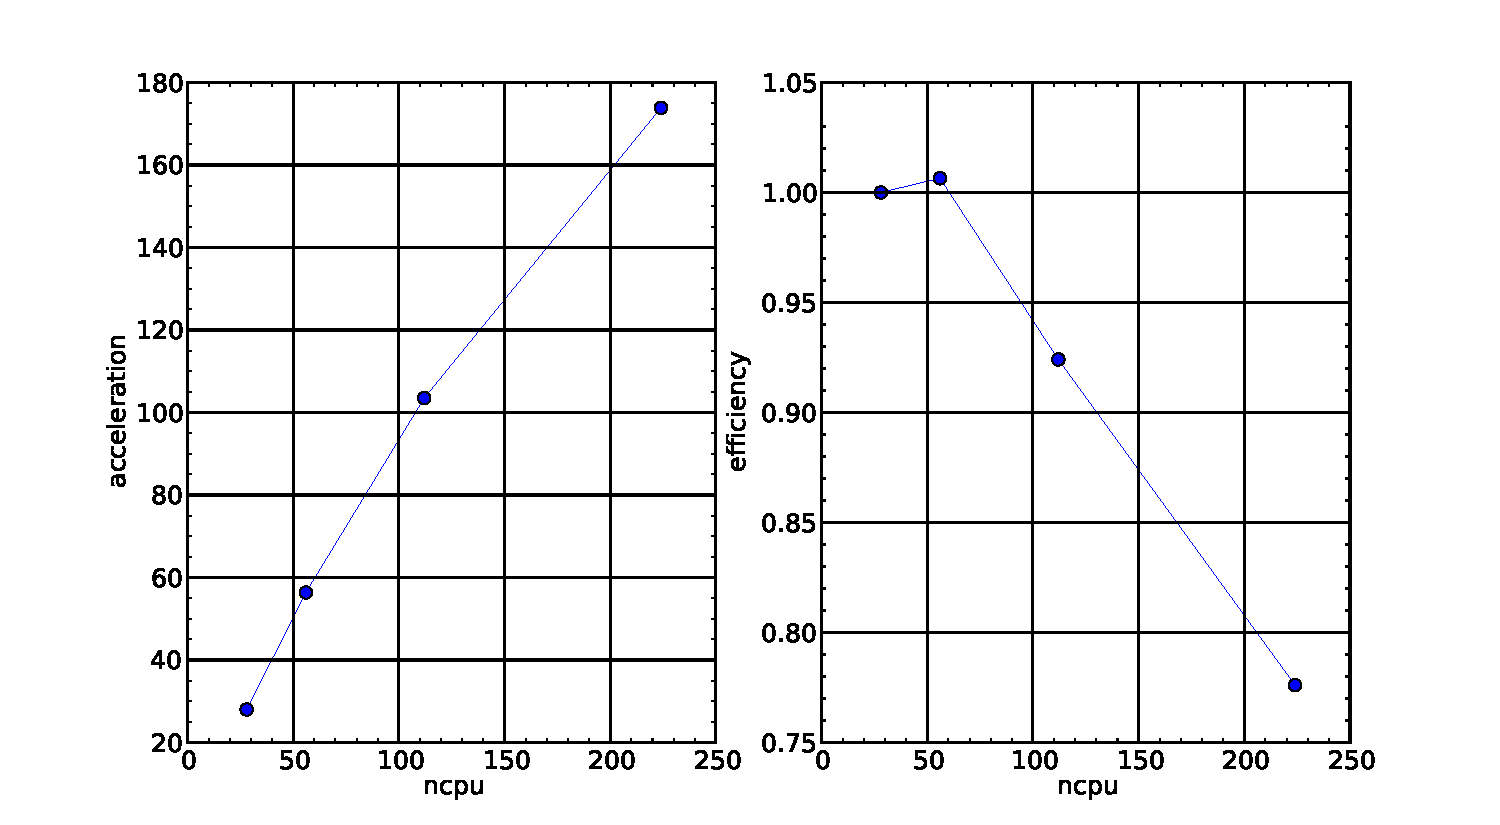
\includegraphics[width=0.49\textwidth]{\figpath/Fig_cap_natconv/Sta_3d_40_scalability.pdf}
%      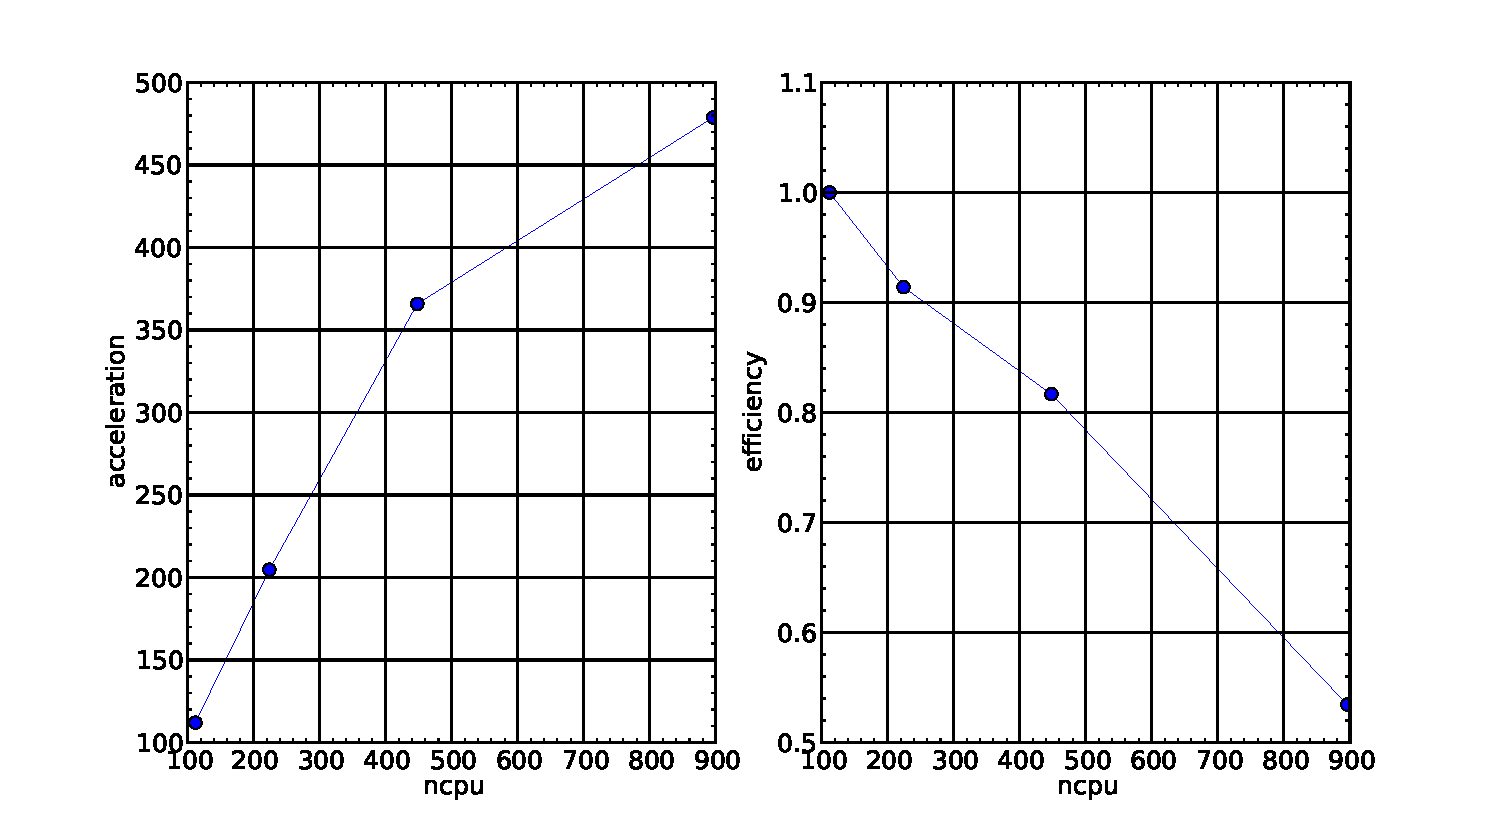
\includegraphics[width=0.49\textwidth]{\figpath/Fig_cap_natconv/Sta_3d_60_scalability.pdf}\\
%      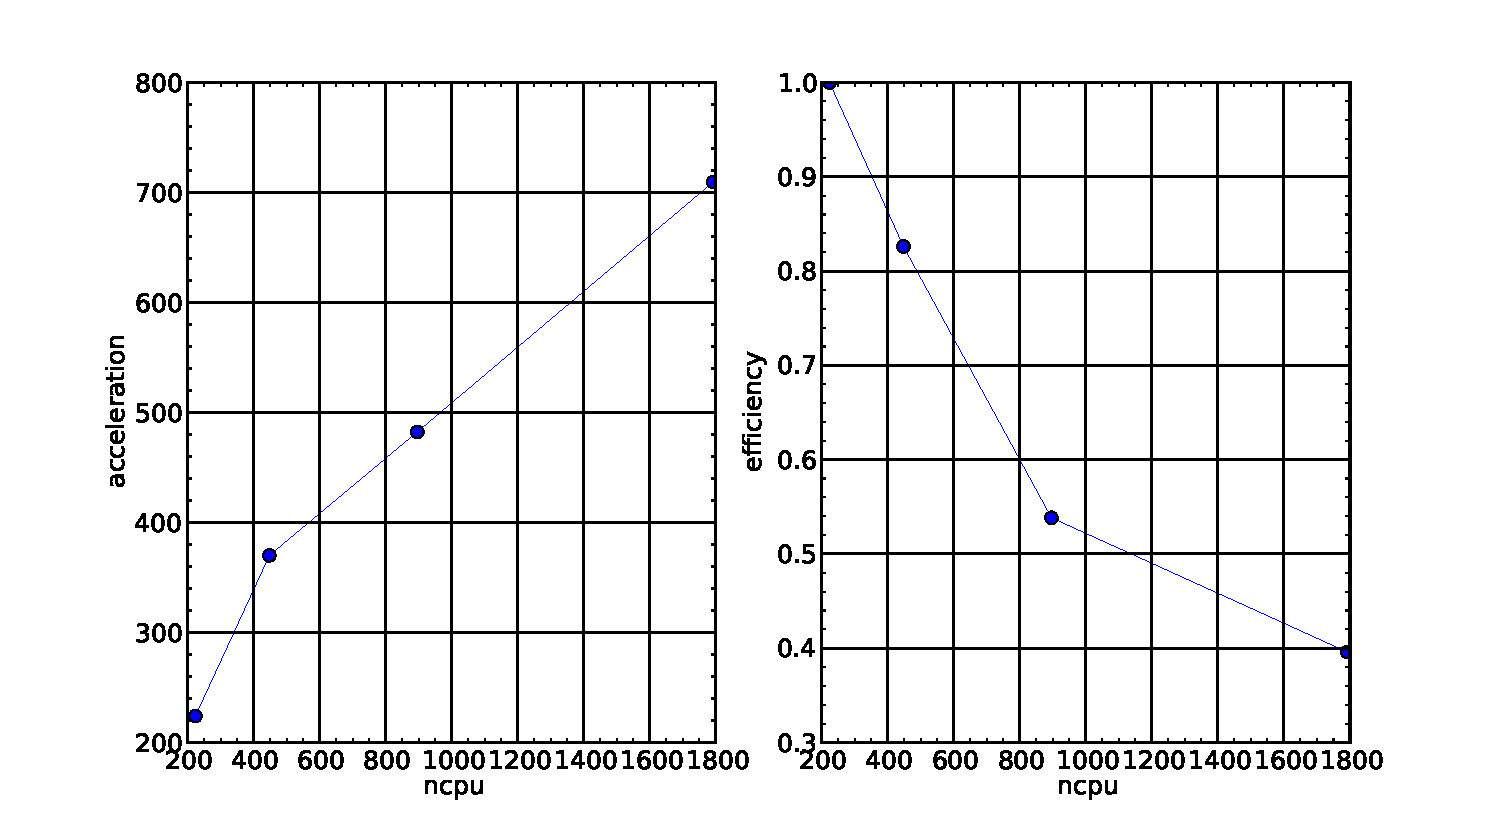
\includegraphics[width=0.49\textwidth]{\figpath/Fig_cap_natconv/Sta_3d_80_scalability.pdf}
%   \end{center}
%   \caption{scalability for a discretisation of $40\times 40$, $60\times 60$ and $80\times 80$}
%   \label{fig-sca_3d_40}
%\end{figure}
%
%\begin{figure}[h]
%   \begin{center}
%      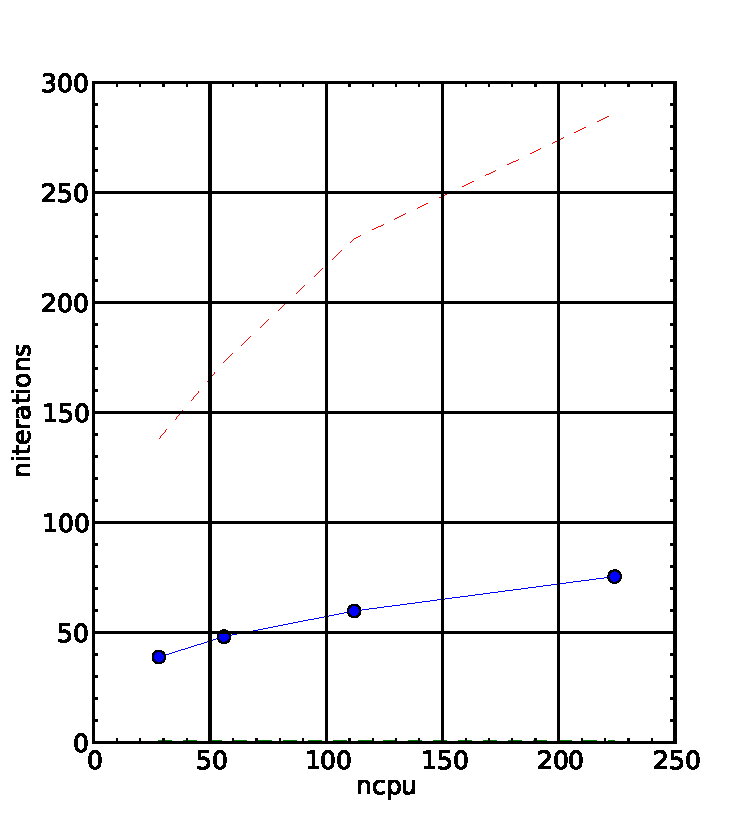
\includegraphics[width=0.3\textwidth]{\figpath/Fig_cap_natconv/Sta_3d_40_gmres.pdf}
%      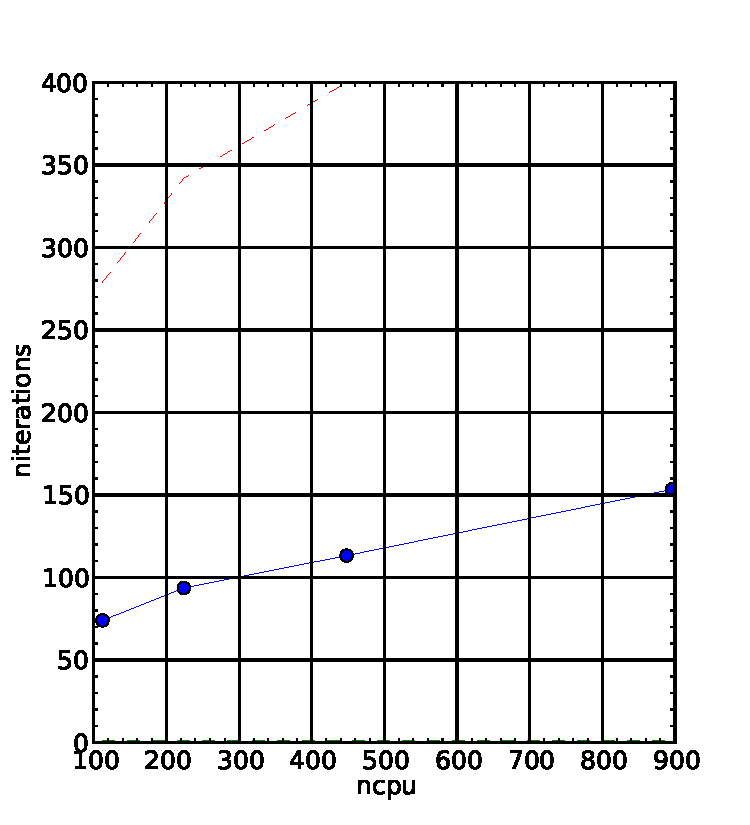
\includegraphics[width=0.3\textwidth]{\figpath/Fig_cap_natconv/Sta_3d_60_gmres.pdf}
%      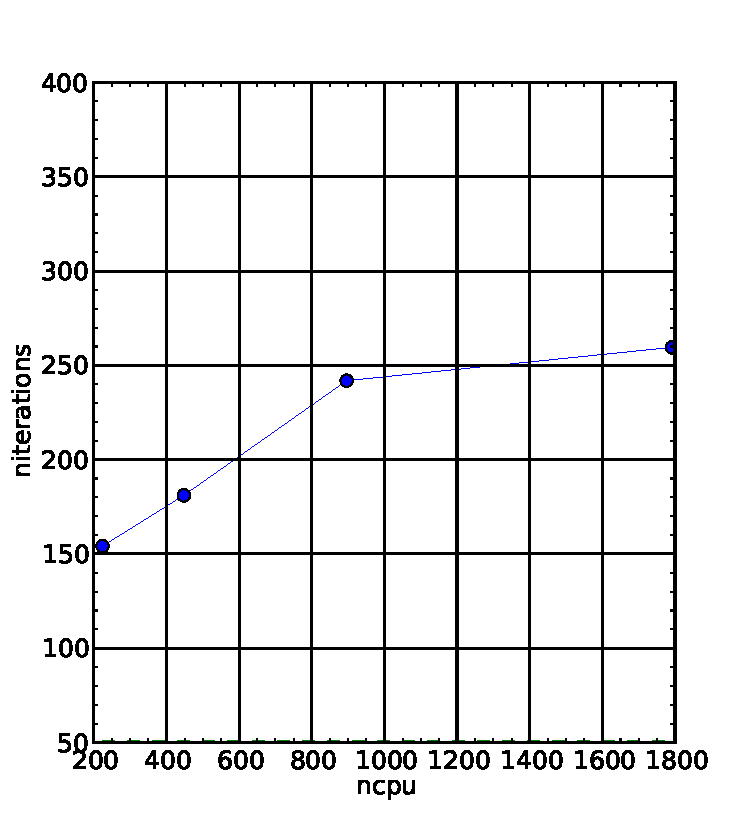
\includegraphics[width=0.3\textwidth]{\figpath/Fig_cap_natconv/Sta_3d_80_gmres.pdf}
%   \end{center}
%   \caption{GMRES iterations for a discretisation of $40\times 40$, $60\times 60$ and $80\times 80$}
%   \label{fig-sca_3d_40}
%\end{figure}



